%% Background
\chapter{Model and System Design}
\label{chap:methodology}

\section{Data Collection}

In order to construct a representative dataset of typeface glyph images, we collected a large number TrueType (.ttf) and OpenType (.otf) binary font files, each of which contains the raw data for an individual typeface or multiple typefaces in one family (Helvetica and Helvetica Light, for example). The majority of our font files (10,682) come from the Capitals64 database constructed by \cite{azadi2017}. We additionally include 3,682 font files from the Google Fonts repository,\footnote{https://github.com/google/fonts/} which contains a wide range of free-to-use fonts accessible in Google applications (Google Docs, Google Slides, etc.) and for downloading, as well as the 64 fonts which come preinstalled with macOS. A complete list of the 14,428 typefaces included in our dataset can be found in the \texttt{fonts.txt} file of our additional resources.

We used the open-source FontForge scripting package\footnote{https://fontforge.org/en-US/} to create an SVG vector image file for each character represented in each typeface. For font files which contained multiple styles in a given font family, we treated each style as a separate typeface, since their respective style representations should be meaningfully different. Before training, we rasterized each SVG file to a $64\times64$ bitmap image.

\section{Models}

Over the course of our research, we employed several model training methods. This section details the various approaches and their respective model architectures. All models were trained in PyTorch 2.4.1 running on a Bizon G7000 G2 GPU server with 2x 32-Core 2.00 GHz Intel Xeon Gold 6338 CPUs and 4x NVIDIA RTX A6000 48 GB GPUs.

\subsection{Basic Autoencoder} \label{basic-autoencoder}

For our first approach, we adapted the original autoencoder model proposed in \cite{rumelhart1986}. An autoencoder, essentially, is a neural network trained to compress and reconstruct input data. A simple diagram of the autoencoder model trained on MNIST data is shown below, in Figure \ref{fig:autoencoder-model}. The autoencoder model consists of two parts: an encoder, which compresses the input data to a smaller vector representation, and a decoder which expands it back out to the original size. Given the capacity of an autoencoder to distill input data, we hypothesized that an autoencoder model trained on font glyph images might generate useful style encodings for typefaces.

% from Bank et al. "Autoencoders"
\begin{figure}[h]
    \centering
    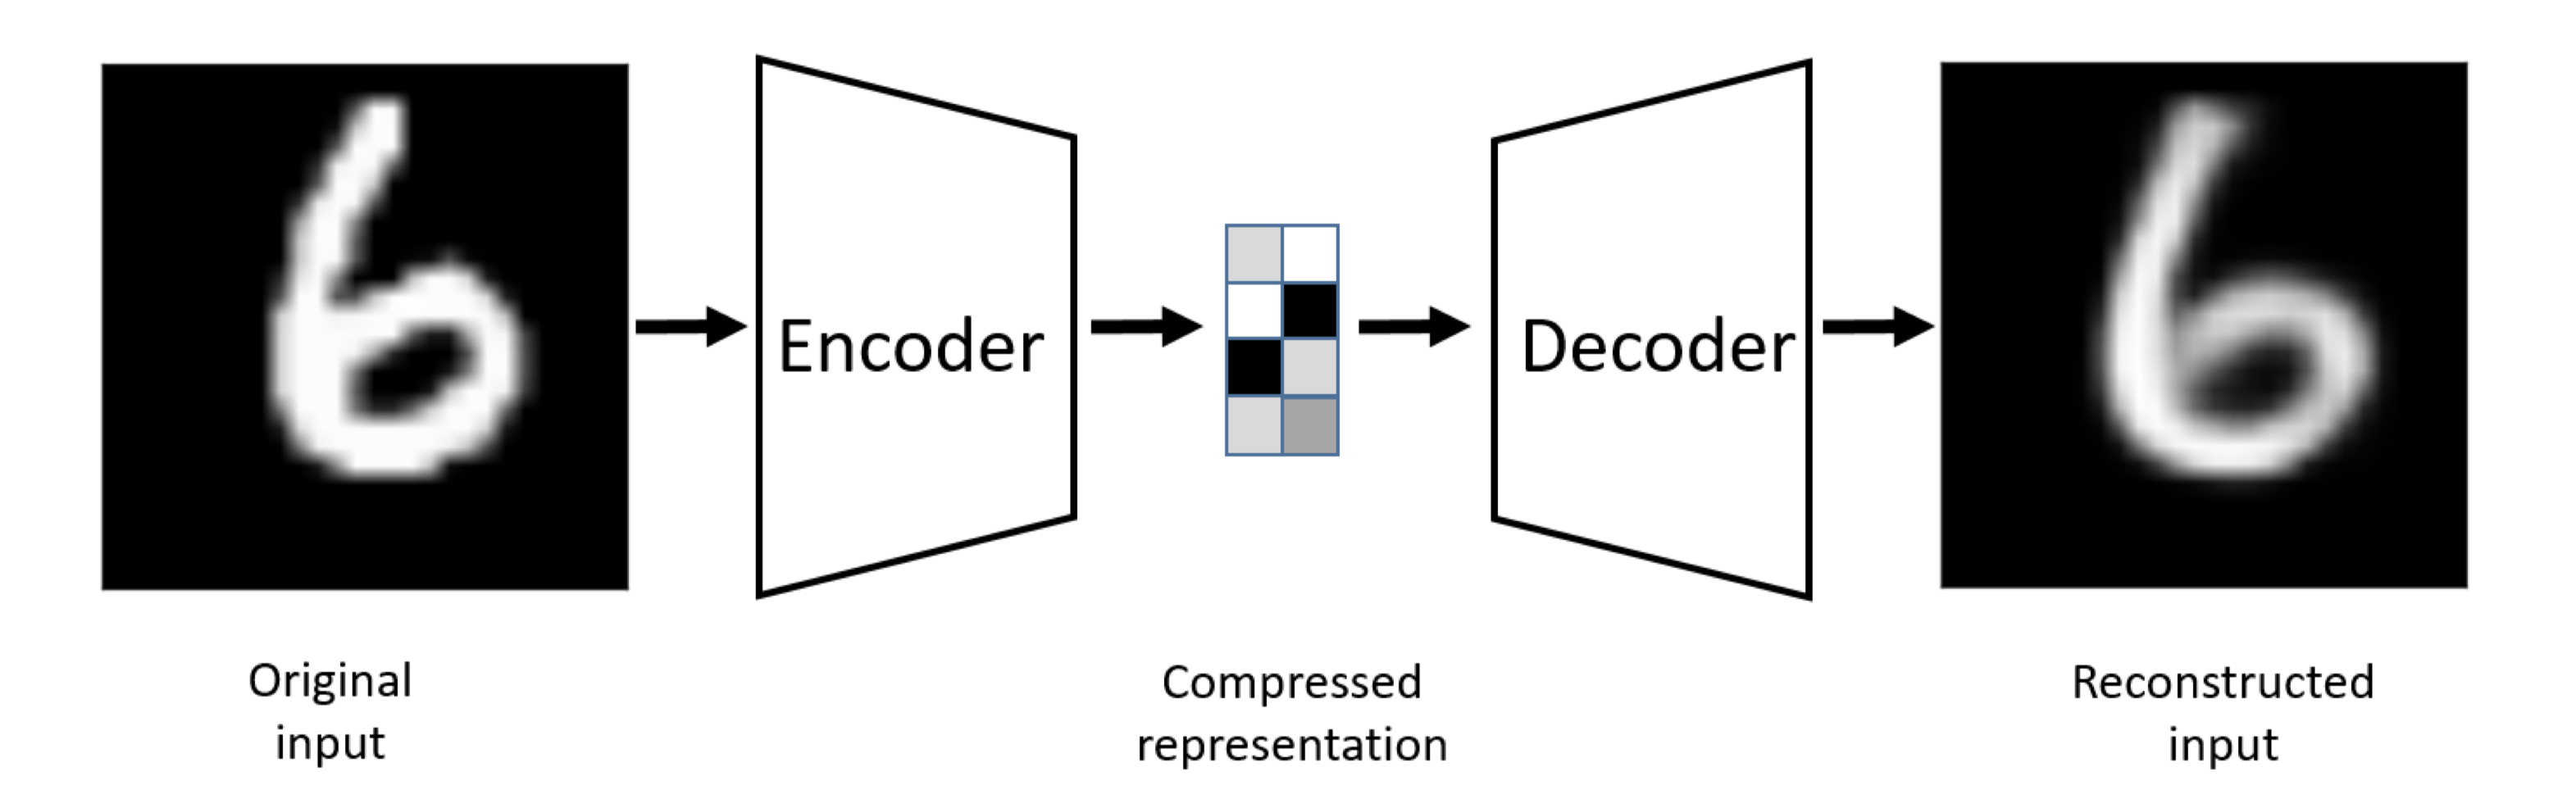
\includegraphics[width=\textwidth]{images/autoencoder-model.png}
    \caption{Basic autoencoder model applied on MNIST data}
    \label{fig:autoencoder-model}
\end{figure}

We implemented an autoencoder model trained to reproduce the glyph images in our database, using a combination of alternating linear layers and ReLU activation functions. Our input data were rasterized character glyphs converted into pixel-intensity matrices, and our model reconstructed output matrices which we translated back into images. We used an MSE loss function, comparing the respective pixel values between the input image and its reconstruction after passing through the autoencoder.

% my own figure
\begin{figure}[h]
    \centering
    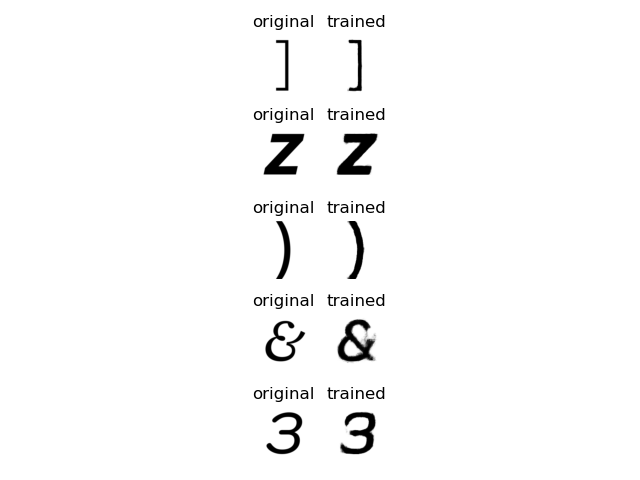
\includegraphics[width=\textwidth]{images/autoencoder-example.png}
    \caption{Our basic autoencoder model inputs/outputs mid-way through training}
    \label{fig:autoencoder-example}
\end{figure}

Some example input and output data from our initial autoencoder model can be found in Figure \ref{fig:autoencoder-example}. However, we quickly realized an issue with this model: given only pixel values as data, the autoencoder has no obvious ability to designate form (the style of a character, defined by its font) from content (the actual letter which is represented). For example, an {\fontspec{Helvetica} A} in Helvetica looks substantively different than an {\fontspec{comicsans.ttf} A} in Comic Sans, but an {\fontspec{Helvetica} A} in Helvetica \textit{also} looks substantively different from a {\fontspec{Helvetica} B} in Helvetica, simply because they are different letters. Our basic autoencoder does not have the necessary data to tell that Helvetica's {\fontspec{Helvetica} A} and {\fontspec{Helvetica} B} should have the same style even though their bitmap representations are different, and that the Comic Sans {\fontspec{comicsans.ttf} A}—whose input data actually looks more similar to the {\fontspec{Helvetica} A} in Helvetica—should have a different style encoding.

\subsection{Style Transfer Autoencoder} \label{style-transfer}

To disentangle this character-style duality, we trained a new modified autoencoder on a different task: to recreate \textit{other} characters in a given font. For example, given an input image of a C character, we trained our model to output a Q character in that same font. We passed two additional vectors into the model as parameters: one representing the character of the input image, and the other representing the target character. By minimizing the MSE difference between the generated character (say, a {\fontspec{Arial} Q} in Arial) and the ground truth glyph in our dataset, we hypothesized that our model would better isolate style in its encodings. Since this model relies on character translation, it was necessary to ensure a common character set across our typefaces. We thus limited our sample size to only include fonts which contained all lowercase (a–z) and uppercase (A–Z) English characters, and trained our style transfer model only on these characters.

Besides the different training tasks, there was a marked difference in our data handling techniques between our style transfer model and the original autoencoder model described in \ref{basic-autoencoder}. First, we had to significantly modify the data loading process: although we were working with a smaller subset of character options (ignoring numbers, punctuation, and special characters), our dataset was in fact larger than in our original autoencoder model. Rather than dealing with every individual character in a font, we needed to handle every \textit{pair} of characters in a font. Since we were using 52 characters per font, we had to train on ${}_{52}C_2 =$ 1,326 character pairs per font. It was necessary to modify our dataloader to provide, for each entry in the dataset, the input truth and output truth images, as well as the input/output characters. Unlike our first autoencoder approach, we also included the input/output characters as parameters inside our model. We created a vector embedding for each; the input embedding was concatenated with the flattened input image data before it was fed through the encoder, and we concatenated the output embedding with the intermediate vector representation between the encoder and decoder steps. Finally, we computed the MSE loss not against the input image but against the ground truth goal image of the target character.

Figure \ref{fig:styletransfer-example} shows our style transfer model part-way through training. The model receives the input {\fontspec{kumar-one.ttf} B} glyph and the input/output character embeddings (not shown), and it attempts to reconstruct the {\fontspec{kumar-one.ttf} h} glyph in the same typeface.

% my own figure
\begin{figure}[h]
    \centering
    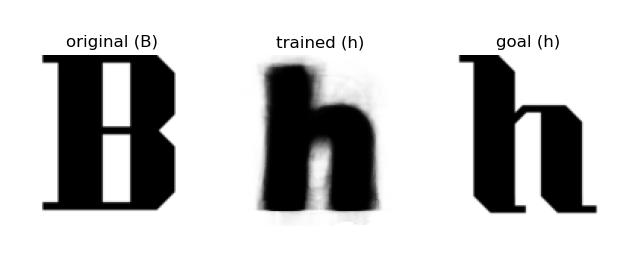
\includegraphics[width=\textwidth]{images/styletransfer-example.png}
    \caption{Example instance of our style transfer model part-way through training}
    \label{fig:styletransfer-example}
\end{figure}

By giving the model explicit vector representation of the input/output characters, we hypothesized that the model would more effectively isolate the style of the glyphs as separate from their content, giving us better internal model embeddings to leverage for typeface style selection.

\subsection{Srivatsan Model}

Our final model, which we adapted from Srivatsan et al. \cite{srivatsan2020}, mirrors our previous approaches in many ways, but it additionally introduces several distinct techniques which may improve the stylistic encoding ability on our dataset. Most notably, the Srivatsan model implements a variational model and uses convolutional layers. It may be necessary to define these terms: a variational model trains to produce intermediate parameters $\mu$ and $\sigma$ of a Gaussian distribution, from which data is randomly sampled before being decoded, rather than training with a fixed intermediate vector encoding. Variational autoencoders (VAEs), proposed by Kingma et. al \cite{kingma2019}, are especially useful for generative tasks in deep learning. A convolutional layer, which can be used in both variational and non-variation models, involves a moving filter called a kernel, which reduces spatial dimensions, improving neural network performance on position-based data like images.

The Srivatsan model, similarly to our Style Transfer model detailed in \ref{style-transfer}, aims at recreating different characters across a typeface and involves vector character embeddings for those input/output characters. However, the model trains on a slightly different task: rather than recreating a specific character in a typeface, the model compiles all input characters for a given typeface (in their case, just the capital letters A-Z) into one image and randomly selects characters to mask. The model is then trained to reproduce these masked characters, using the latent style embedding and the respective character embedding for the masked glyphs. A diagram of the Srivatsan model architecture can be found in Figure \ref{fig:srivatsan-model}.

% my own figure
\begin{figure}[h]
    \centering
    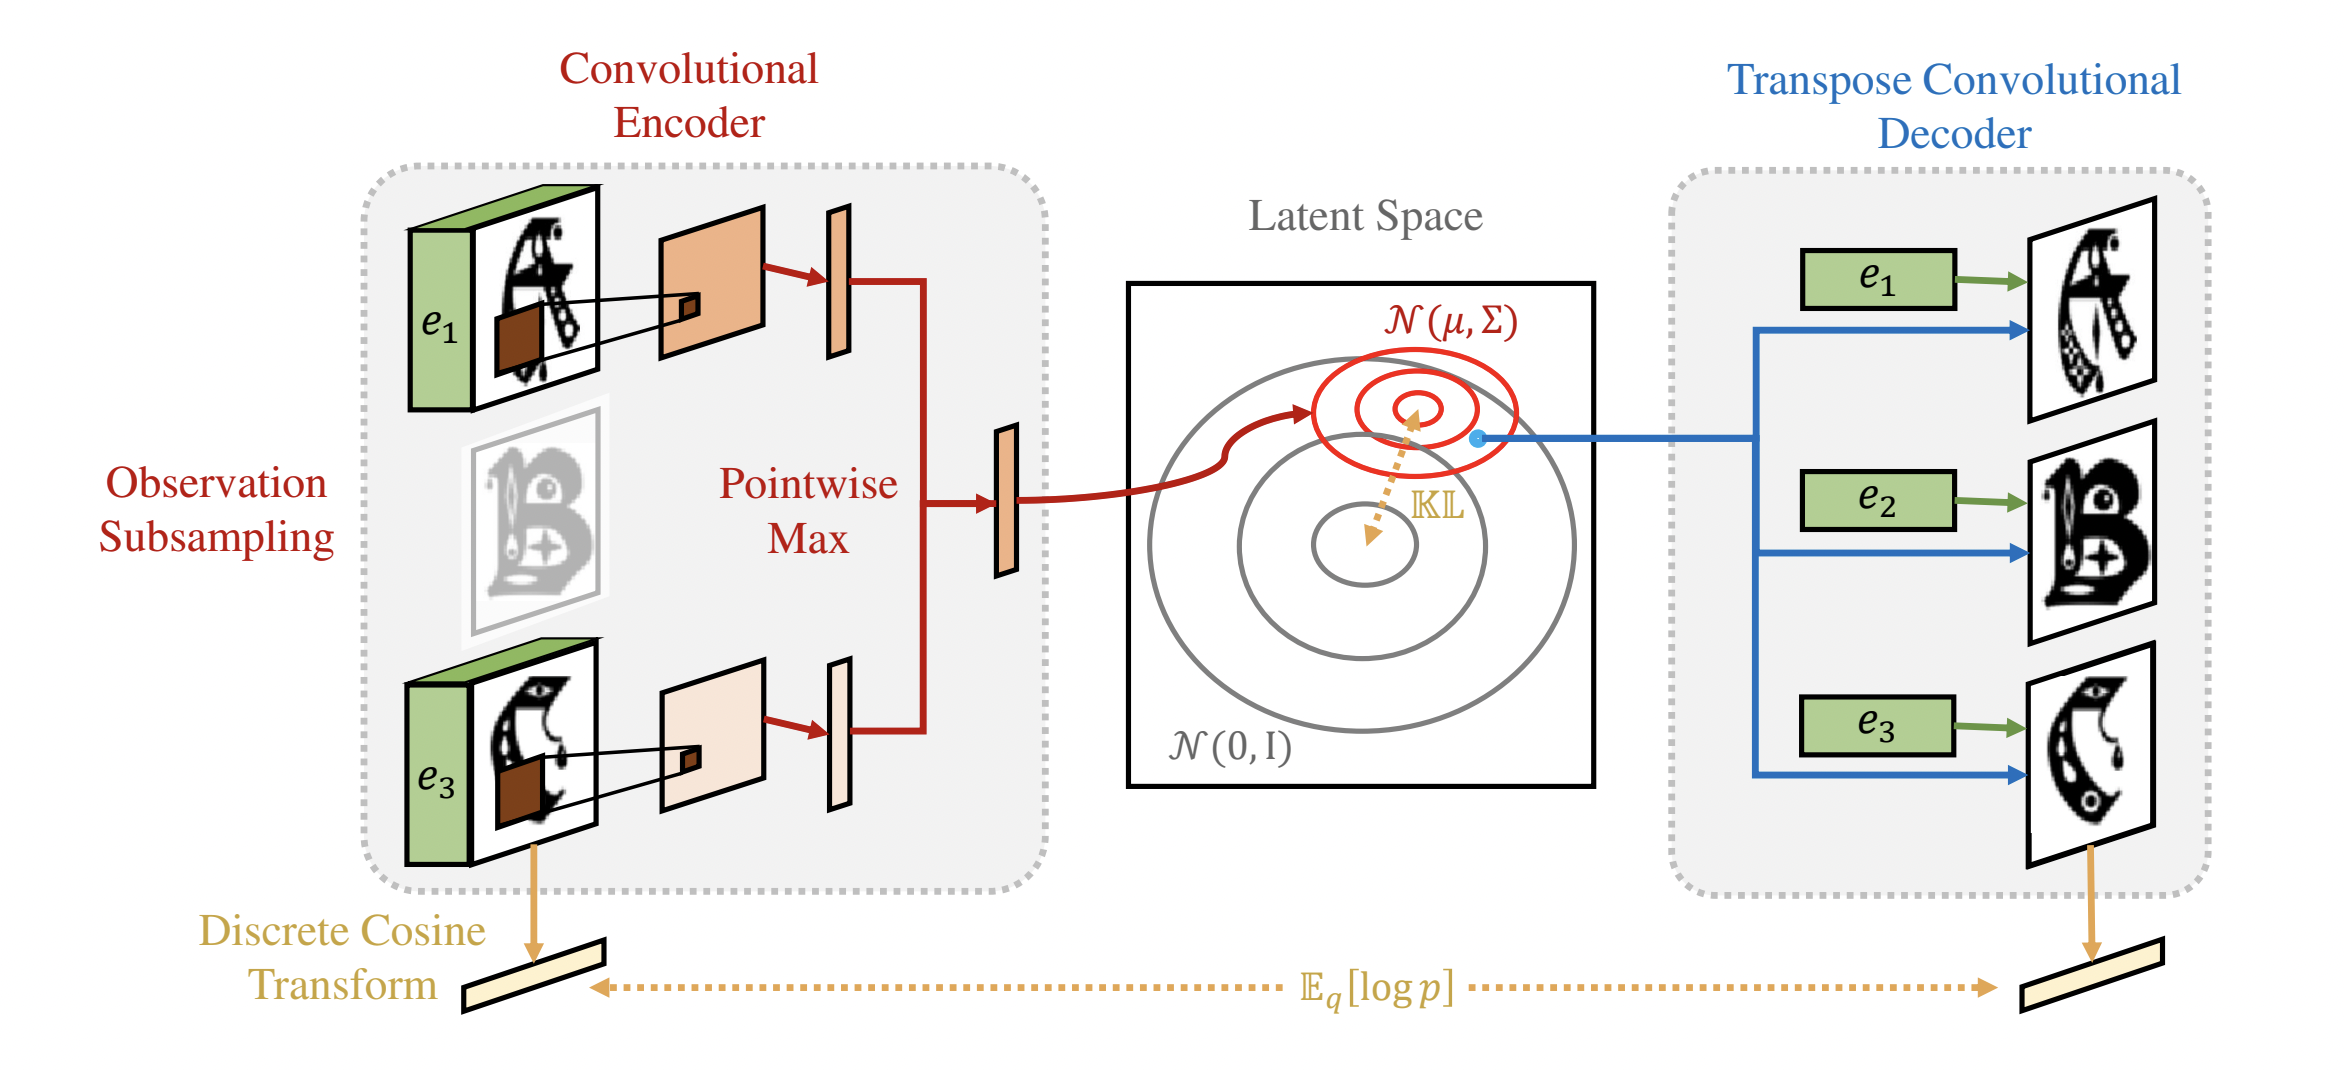
\includegraphics[width=\textwidth]{images/srivatsan-model.png}
    \caption{Diagram of Srivatsan et al. model architecture}
    \label{fig:srivatsan-model}
\end{figure}
 
Srivatsan et al. does an adequate job at glyph reconstruction–one of the focuses of the paper—but it excels especially at generating style encodings. Figure \ref{fig:srivatsan-tsne} shows a t-SNE plot of the latent style encodings generated by the Srivatsan model, colored by both weight and Google Font style category. As the figure shows, it is quite effective at encoding both the weight of a font (bolder or lighter) and the more ambiguous aspects of its style, shown in the coarse style categories from Google Fonts.

% my own figure
\begin{figure}[h]
    \centering
    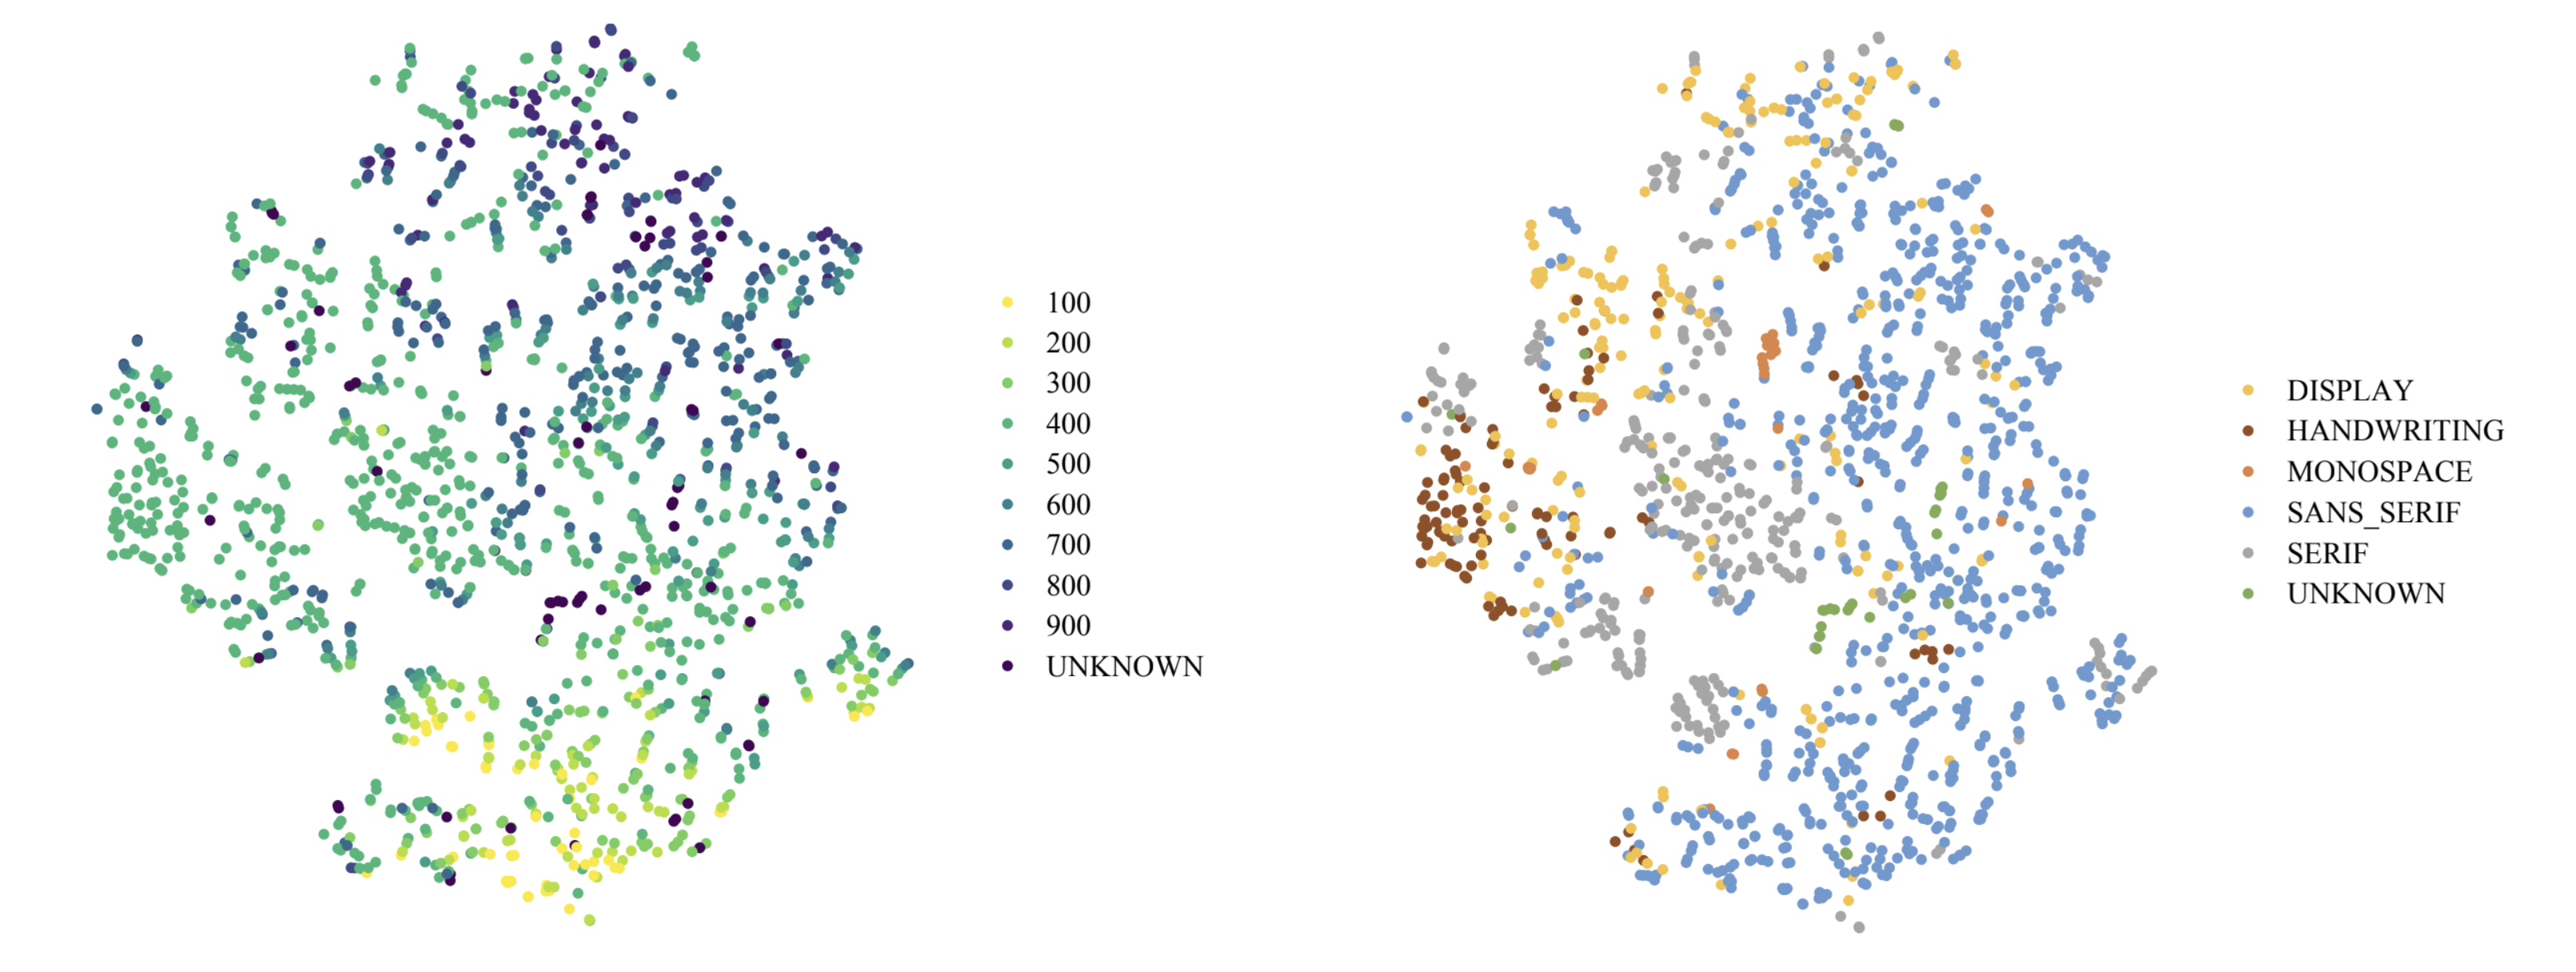
\includegraphics[width=\textwidth]{images/srivatsan-tsne.png}
    \caption{t-SNE plot of style encodings from Srivatsan et al. colored by weight (left) and Google Font style category (right)}
    \label{fig:srivatsan-tsne}
\end{figure}

We ported the original code from Srivatsan et al. from Python 2.7 and PyTorch 1.1.0 to Python 3.13 and PyTorch 2.5.1 and trained it using their original Capitals64 dataset. However, after training we ran the model on a modified version of our Google Fonts dataset in order to generate useful style encodings which we could compare with our other models.

\subsection{Extracting Style Encodings}

In order to build useful typeface selection tools based on these models, it was necessary in all three cases to extract the model's internal style encoding vector for each typeface. This task was relatively trivial for the first two models: we simply passed each of the typeface character sets through the encoder portion of our model and performed an elementwise average across the resulting vector representation for each character. For the Srivatsan model, we similarly ran our model on each of the typeface character sets; however, since the Srivatsan model applies a variational approach, it was additionally necessary to perform a random sample from the Gaussian distribution defined by each typeface character set to obtain a style encoding. Because the architecture of the Srivatsan model does not train on individual character sets or pairs, but entire typeface character sets at once, it was not necessary to take an average of multiple character style encodings; the model, by design, trains one generalized latent style encoding for each typeface.

\section{System Design}

In this section, we detail the process and design of turning our style encodings—generated by the models in the previous section—into a user tool for typeface selection. We consider questions of encoding dimensionality, end-to-end system design, and user experience in order to create a novel, useful typeface selector tool.

\subsection{Style Encoding Dimensionality}

One initial question which emerges when training autoencoder-like models, especially with the goal of extracting intermediate encoding vectors, is: what should be the dimensionality of those encodings? In our case especially, there is a tradeoff between encoding more information (higher dimensional vectors should be able to represent greater stylistic detail, to a certain point) and usability (lower dimensional vectors represent fewer choices for users, presumably yielding easier-to-use tools). One could, for example, train a model to generate 2-dimensional style encodings; this could create a very useful tool—we could represent this as a scatterplot of typefaces or as two sliders corresponding to the two style axes—but two dimensions is not very much space to represent the many diverse axes of typeface style. Alternatively, one could choose a very high dimensional style encoding—say, a 100-dimensional vector—which would have a much greater capacity to encode the many axes of font style; however, presenting a user with a decision for each of those dimensions would be an unwieldly and overwhelming experience for most.

We tested several embedding dimensions, but ultimately chose to encode typeface style in 6-dimensional vectors across our three models. This provides significant room for spatial exploration of typeface style, but also reasonably limits user choice, creating a better user experience. In the following section, we will describe how these six dimensions translate to a novel font selection tool; additionally, we compress these 6-dimensional style encodings into 2-dimensional space using t-SNE reduction to create an auxilliary scatterplot tool which provides users with an additional, more familiar graphical representation of the data.

\subsection{User Experience}

We experimented with several iterations of a tool which would allow users to interact with higih-dimensional style encodings in a useful manner. As mentioned previously, the question of dimensionality is a significant one when generating style encodings for user interaction; another important consideration is \textit{how} users should interact with these high-dimensional vector spaces. Should users have full control over each dimension, or should they be guided in their decisions? How should high-dimensional space—which cannot be easily visualized or conceptualized by users—be represented? What additional tools should be provided to users (a back button, the ability to save a typeface for later reconsideration, a search bar) would help a user navigate this high-dimensional stylistic vector space? Other relevant user design questions are: What is the goal of our user (finding a specific font, finding similar fonts to a given font, or open exploration)? How much time is the user willing to spend searching for a font? What does the user want to do with this font (or fonts) once identified, and how can we assist the user to accomplish that?

% my own figure
\begin{figure}[h]
    \centering
    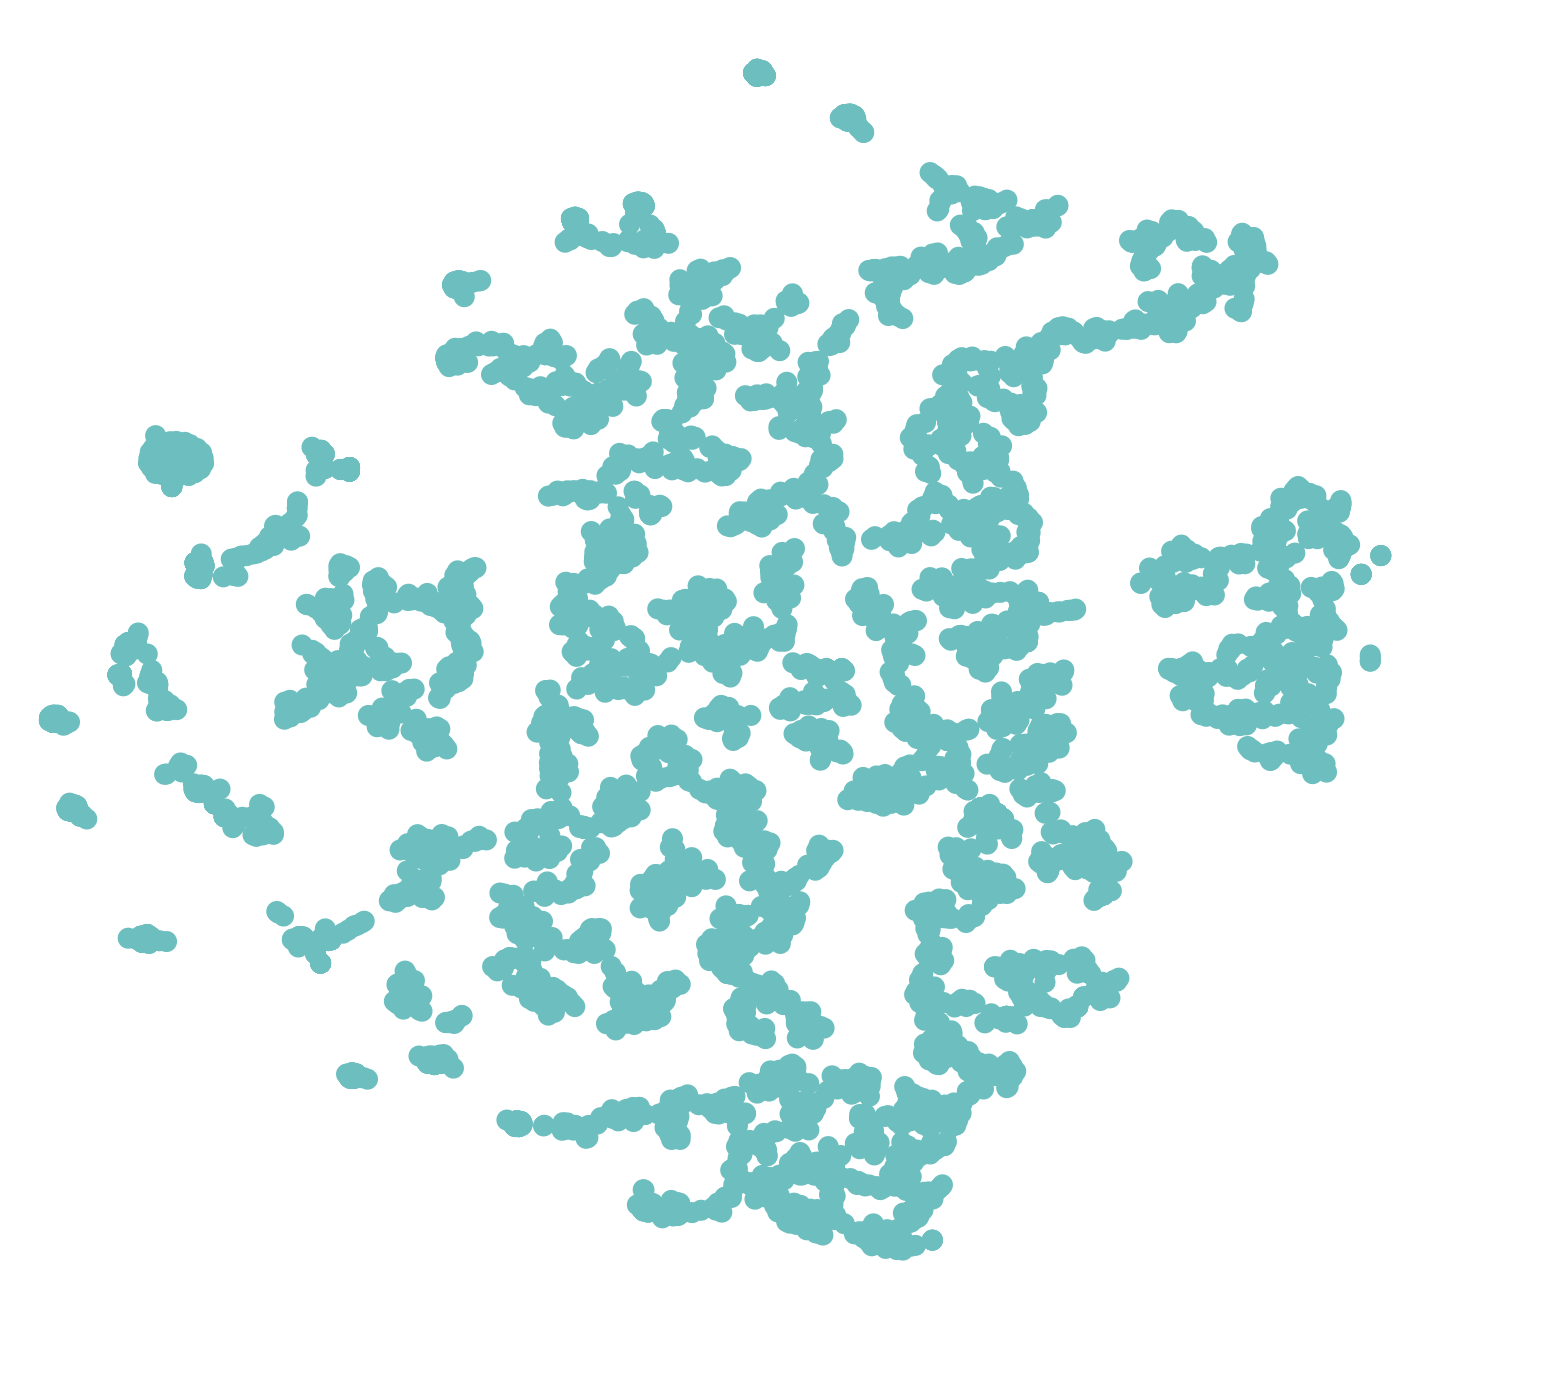
\includegraphics[width=270pt]{images/scatterplot-tool.png}
    \caption{t-SNE scatterplot of our style encodings, allowing users to visually navigate a reduced-dimensionality version of our model style encodings}
    \label{fig:scatterplot-tool}
\end{figure}

The current iteration of our typeface selector tool involves two connected user tools which allow users to explore our 6-dimensional vector style space in two complementary ways. The first tool (Figure \ref{fig:scatterplot-tool}) is an interactive scatter plot, displaying a t-SNE reduction of our 6-dimensional style space. t-SNE is a dimensionality reduction technique which preserves local structure and clustering, meaning that typefaces which are near each other in the original 6-dimensional representation generally remain near to each other in the reduced 2-dimensional space. The scatterplot is an intuitive and familiar representation of spatial data to most users, making it a useful tool for navigating this style-embedding space. Users can explore the scatterplot space and visualize the fonts represented at each point; if a user identifies a font that is similar to the font they are searching for or imagining, they should be able to find other, even more similar fonts by exploring the points nearby. 

% my own figure
\begin{figure}[h]
    \centering
    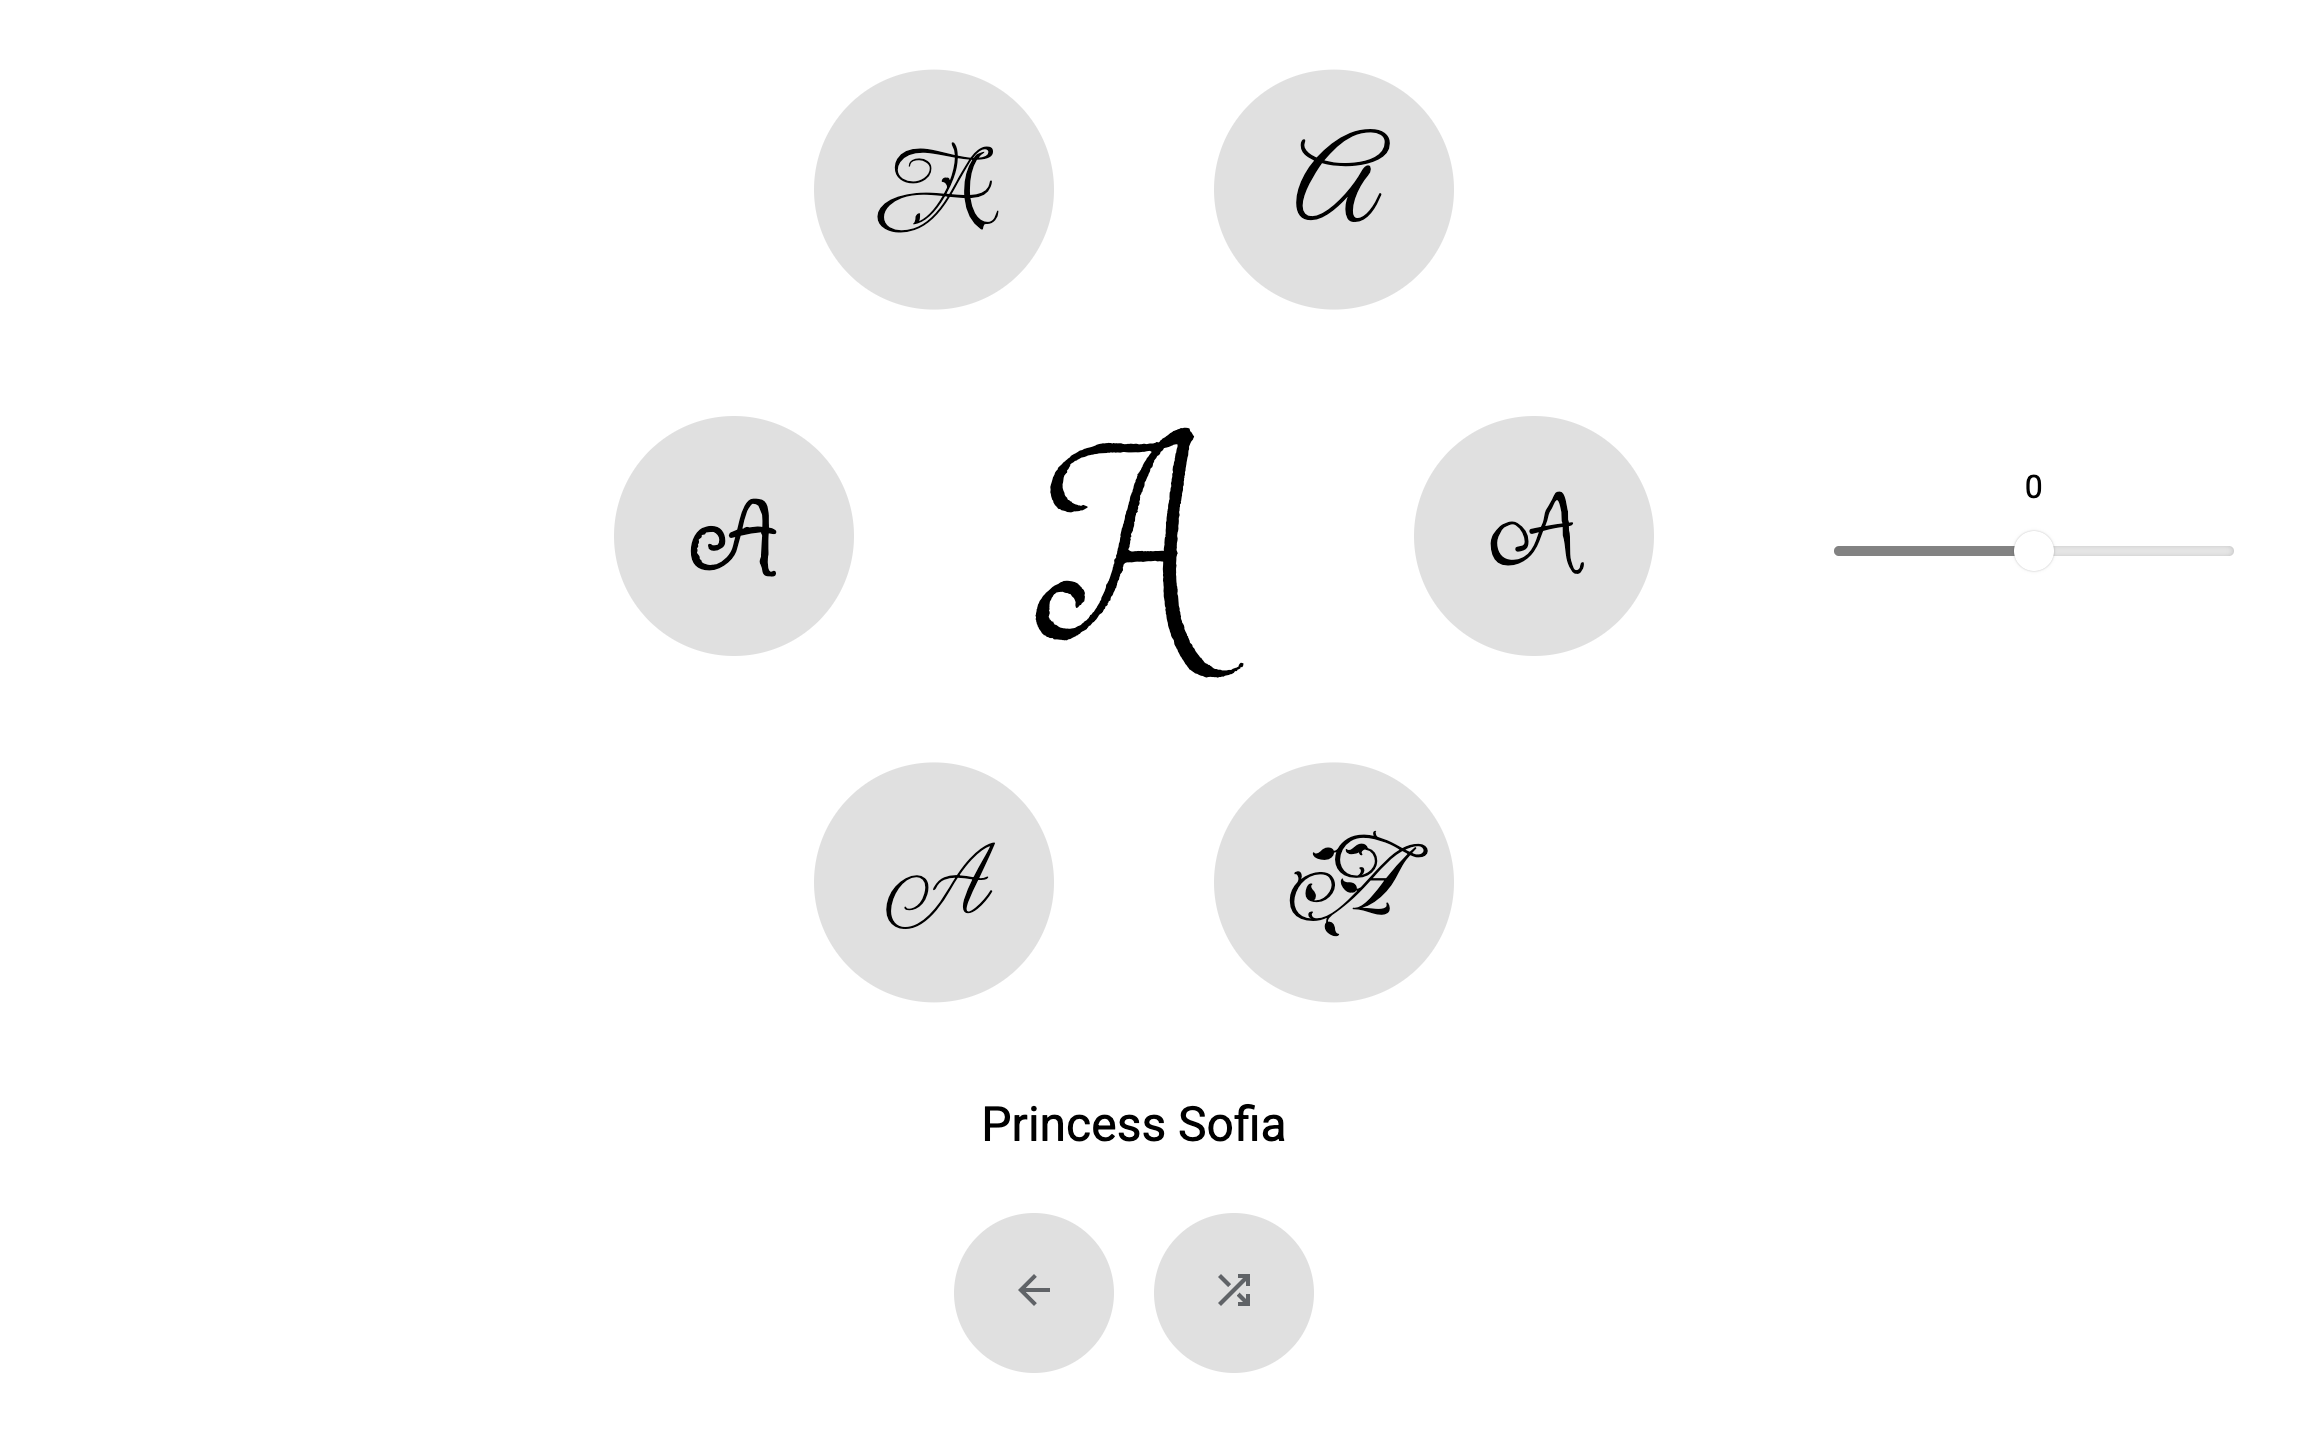
\includegraphics[width=\textwidth]{images/selector-tool.png}
    \caption{Our novel 6-dimensional typeface selector tool}
    \label{fig:selector-tool}
\end{figure}

In order to provide another way for users to interact with this style space—one which preserves the dimensionality of our style encodings and therefore allows users full range over the model space—we propose another typeface selector tool based on the 6-dimensional structure of our encoding data. This tool, shown in Figure \ref{fig:selector-tool}, displays a center font glyph (A is the default character, but this can be changed by the user) of a randomly-selected typeface in the model space, and shows the six nearest neighbors of that font (determined by Euclidean distance) in a circle surrounding it. The slider, on the right hand side, represents magnitude; when the magnitude is zero, the six surrounding fonts represent the nearest neighbors to the center font; when the magnitude is nonzero, the tool will search—along all six dimensions of the model space—according to the distance defined by the slider magnitude, and display the closest font in each of those dimensions. Therefore, as the slider grows further from zero, the six fonts displayed will have increasingly different style from the center font. At any point, a user can select one of the six surrounding fonts and move to that point in the model space, at which point the slider resets to zero (nearest neighbor), and the user may continue the process again in order to find a more optimal font. The tool also includes a shuffle button, enabling the uer to randomly select a new font, and a back button which allows the user to return to previously seen fonts. By providing easy-to-use buttons and dynamically displaying fonts, this tool enables users to navigate a high-dimensional model space which is difficult to conceptualize intuitively.

% my own figure
\begin{figure}[h]
    \centering
    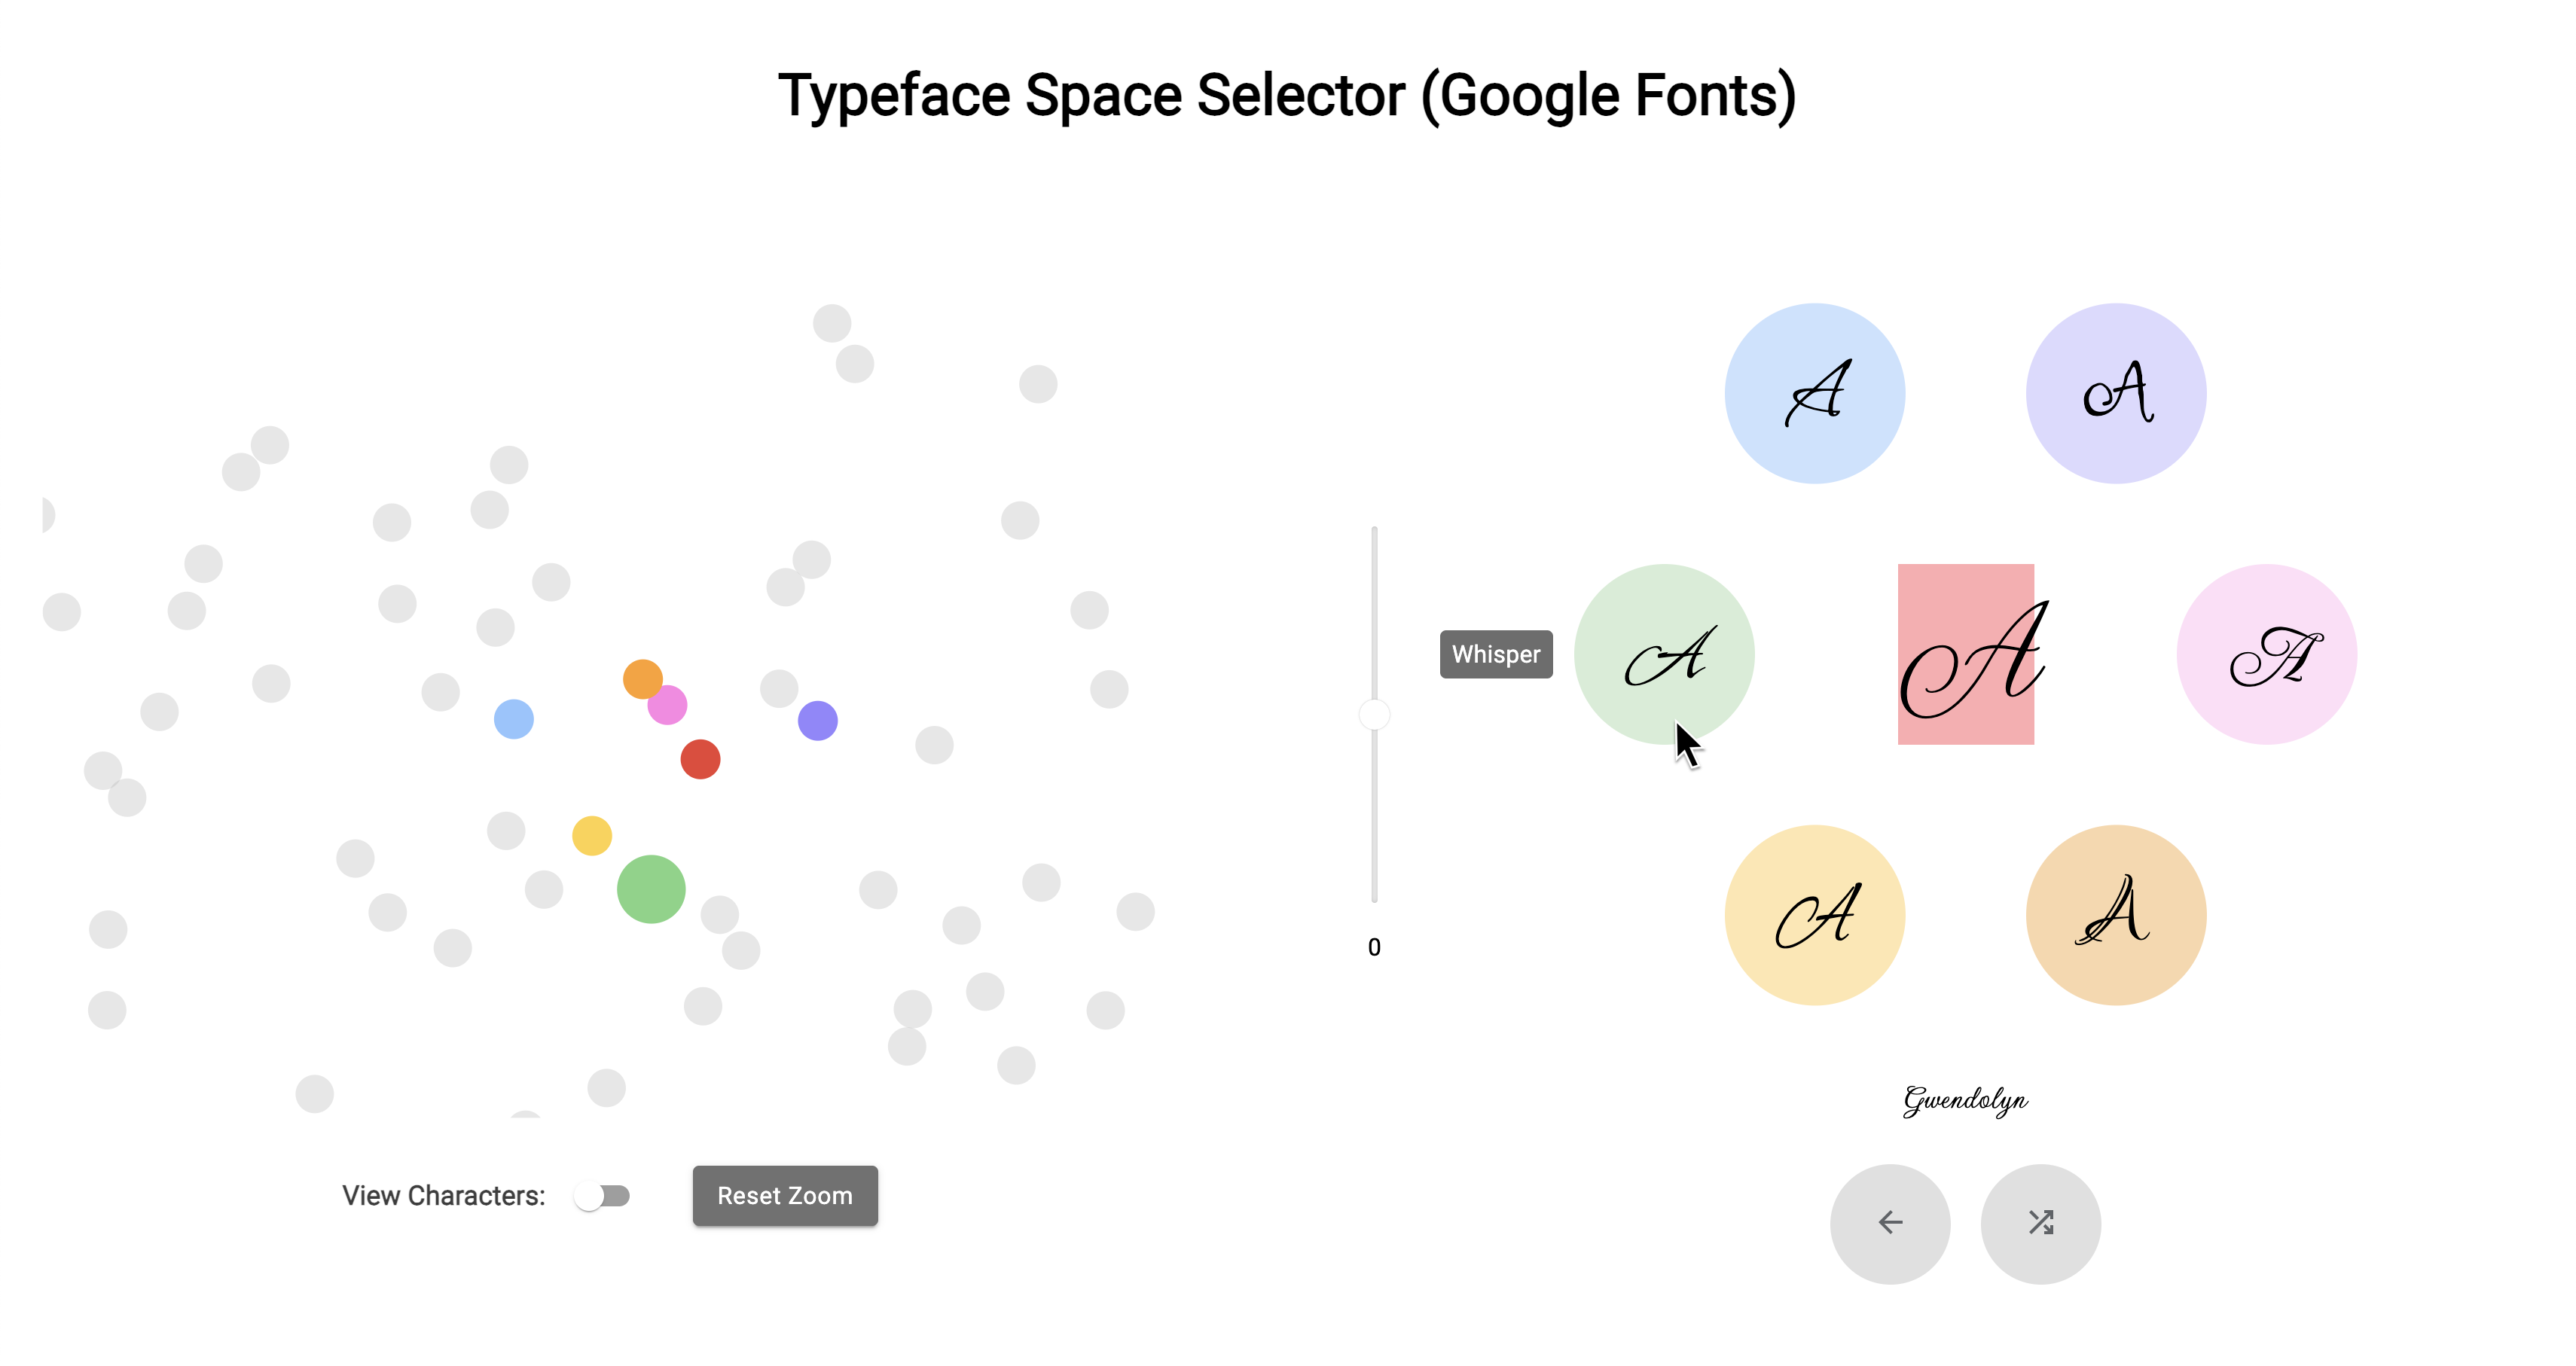
\includegraphics[width=\textwidth]{images/both-selectors.png}
    \caption{Both of our typeface selector tools side-by-side, allowing use of both tools in tandem}
    \label{fig:both-selectors}
\end{figure}

Our final product combines both the scatterplot and six-point tool. Users can alternate between the two to take advantage of the respective features of each tool. In order to make our implementation more streamlined, this font selector is currently limited to the Google Fonts collection of typefaces. (This choice is described further in \ref{frontend}.)

\subsection{Backend}

We implement the backend of our web app in Flask,\footnote{https://flask.palletsprojects.com/en/stable/} a lightweight Python web server which adds expands capability on top of the basic HTTP GET and POST requests and includes support for URL parameters. The backend server provides two functionalities: serving t-SNE data and performing nearest-neighbor calculations. In the first case, the backend serves the full t-SNE dataset for use in our scatterplot selector tool (a small file <1MB) upon request from the frontend web app. As its second function, the server can be queried to navigate the 6-dimensional model space and compute the nearest neighbor calculations necessary for the six-point font selector tool. This backend computation—built on the Facebook AI Similarity Search (FAISS) library,\footnote{https://ai.meta.com/tools/faiss/} which provides efficient, high-dimensional vector similarity search—is as follows: given an input typeface and magnitude, the server first locates the style encoding for the input typeface, then creates six new style encoding vectors with the magnitude value added in each of the corresponding dimensions. FAISS then finds the nearest actual typeface style encoding for each of the six calculated vectors (avoiding duplicates when possible) and serves those font names to the client in a JSON file.

\subsection{Frontend} \label{frontend}

Our frontend is implemented in React,\footnote{https://react.dev/} an open-source JavaScript library built to create interactive web applications using modular components. The scatterplot tool uses the Chart.js library\footnote{https://www.chartjs.org/} for simple, efficient plot creation, and the 6-point font selector was built by hand using React components. For rendering the actual fonts, our frontend uses the GoogleFontLoader package for React,\footnote{https://www.npmjs.com/package/react-google-font-loader} which facilitates easy, dynamic font loading on webpages. This allows us to avoid serving the 2.7GB of font binary files, alleviating significant server load; however, it limits our current implementation to typefaces from the Google Fonts library. This is not necessarily a bad thing—Google Fonts is widely-used and contains a wide range of different fonts—but it does mean that common proprietary fonts such as Times New Roman and Comic Sans are also not included in the current version of our font selector tool.